\chapter{Bài 5. Chuyển động tổng hợp}
\begin{center}
	\textit{(3 tiết)}
\end{center}
\section{MỤC TIÊU DẠY HỌC}
\begin{center}
	\begin{longtable}{|M{2.5cm}|L{12.5cm}|M{2cm}|}
		\hline
		\thead{Biểu hiện\\ năng lực} & \thead{Mục tiêu} & \thead{STT}\\
		\hline
		\multicolumn{3}{|c|}{\textbf{ Năng lực vật lí}}\\
		\hline
		1.1 & Phát biểu được tính tương đối của chuyển động và vận tốc, từ đó thấy được tầm quan trọng của hệ quy chiếu. & 1\\
		\hline
		1.4 & Phân biệt được hệ quy chiếu chuyển động và hệ quy chiếu đứng yên. & 2\\
		\hline
		1.2&Xác định được độ dịch chuyển tổng hợp, vận tốc tổng hợp. & 3\\
		\hline
		\multicolumn{3}{|c|}{\textbf{Năng lực chung}}\\
		\hline
		TC - TH& Tích cực thực hiện các nhiệm vụ GV đặt ra cho các nhóm, tích cực suy luận để đưa ra câu trả lời trong quá trình GV định hướng nội dung học tập	&4 \\
		\hline
		GT - HT & Tích cực đóng góp ý kiến trong quá trình thảo luận, biết sử dụng ngôn ngữ kết hợp với các loại phương tiện phi ngôn ngữ đa dạng để trình bày các kết quả thảo luận nhóm & 5\\
		\hline
	\end{longtable}
\end{center}
\section{THIẾT BỊ DẠY HỌC VÀ HỌC LIỆU}
\begin{itemize}
	\item Tivi/máy chiếu;
	\item SGK;
\end{itemize}
\section{TIẾN TRÌNH DẠY HỌC}
\subsection{TIẾN TRÌNH}\newpage
\begin{center}
	\begin{longtable}{|L{2.75cm}|C{1.25cm}|L{5cm}|L{3.5cm}|L{4cm}|}
		\hline
		\thead{Tiến trình} & \thead{Mục\\tiêu} & \thead{Nội dung dạy học \\trọng tâm} & \thead{PP,\\ KTDH} & \thead{Phương pháp \\đánh giá}\\
		\hline
	\textbf{Hoạt động 1:} Tìm hiểu về tính tương đối của chuyển động	& 1, 2  & Tính tương đối của chuyển động. Phân biệt hệ quy chiếu chuyển động và hệ quy chiếu đứng yên.  & PPDH: Đàm thoại & GV đánh giá dựa trên câu trả lời của HS.\newline
	PP đánh giá: quan sát, nghe.  \\
		\hline
		\textbf{Hoạt động 2:} Tìm hiểu độ dịch chuyển tổng hợp - vận tốc tổng hợp. & 3 & Độ dịch chuyển tổng hợp, vận tốc tổng hợp & PPDH: Đàm thoại &  GV đánh giá dựa trên câu trả lời của HS.\newline
		PP đánh giá: quan sát, nghe.  \\
		\hline
		\textbf{Hoạt động 3:} Vận dụng quy tắc cộng vector để tìm vận tốc tổng hợp trong các trường hợp đơn giản. & 3, 4, 5 & Công thức vận tốc tổng hợp trong trường hợp: \begin{itemize}
			\item $\vec{v}_{12}\uparrow\uparrow \vec{v}_{23}$; \item $\vec{v}_{12}\uparrow\downarrow \vec{v}_{23}$; \item $\vec{v}_{12}\bot\vec{v}_{23}$
		\end{itemize}& PPDH: Dạy học hợp tác & GV đánh giá dựa trên câu trả lời đại diện nhóm HS.\newline
		PP đánh giá: quan sát, nghe.  \\
		\hline
		\textbf{Hoạt động 4:} Luyện tập	& 1, 2, 3  & Luyện tập bài tập vận tốc tổng hợp, bài toán thuyền chạy xuôi dòng/ngược dòng. & PPDH:  Đàm thoại& GV đánh giá dựa trên bài tập cá nhân của học sinh.\newline
		PP đánh giá: quan sát, nghe. \\
		\hline
		\end{longtable}
\end{center}
% ==========================================================================================
\hoatdong
{Tìm hiểu về tính tương đối của chuyển động.	
}
{\begin{itemize}
		\item HS phát biểu được tính tương đối của chuyển động và vận tốc, từ đó thấy được tầm quan trọng của hệ quy chiếu.
		\item HS phân biệt được hệ quy chiếu chuyển động và hệ quy chiếu đứng yên.
	\end{itemize}
	
}
{
		Kết quả trả lời của HS cho các câu hỏi gợi mở của GV:\\
	\textbf{Câu trả lời dự kiến:} 
	\begin{itemize}
		\item Câu hỏi 1: Khi bánh xe đạp quay, quỹ đạo chuyển động của đầu van so với trục ổ bi có hình dạng gì?\\
		Trả lời: quỹ đạo tròn.
		\item Câu hỏi 2: Đối với người quan sát bên đường, đầu van xe đạp chuyển động với quỹ đạo thế nào?\\
		Trả lời: quỹ đạo như một nửa đường xoắn ốc (cycloid).
		\item Câu hỏi 3: Nhận xét trạng thái chuyển động của hành khách so với tài xế và cây xương rồng bên đường.\\
		Trả lời: Hành khách đứng yên so với tài xế nhưng đang chuyển động so với cây bên đường.
	\end{itemize}
}
{\textit{\underline{* GV chuyển giao nhiệm vụ học tập}}\\
	GV lần lượt đặt các câu hỏi gợi mở cho HS.\\
	\textbf{Câu 1:} Khi bánh xe đạp quay, quỹ đạo chuyển động của đầu van so với trục ổ bi có hình dạng gì?
	\begin{center}
		\includegraphics[width=0.4\linewidth]{figs/G10-BAI5-1}
	\end{center}
	\textbf{Câu 2:} Đối với người quan sát bên đường, đầu van xe đạp chuyển động với quỹ đạo thế nào?
	\begin{center}
		\includegraphics[width=0.4\linewidth]{figs/G10-BAI5-2}
	\end{center}
	\textbf{Câu 3:} Nhận xét trạng thái chuyển động của hành khách so với tài xế và cây xương rồng bên đường.
	\begin{center}
		\includegraphics[width=0.4\linewidth]{figs/G10-BAI5-3}
	\end{center}
	\textit{\underline{* HS thực hiện nhiệm vụ học tập}}\\
	HS tích lắng nghe, suy nghĩ.\\
	\textit{\underline{* HS báo cáo kết quả nhiệm vụ học tập}}\\
	HS tích cực trả lời câu hỏi gợi mở của GV.\\
	HS chú ý theo dõi, đặt câu hỏi.\\
	GV chỉnh lí, hợp thức hóa kiến thức.
}
% ==========================================================================================
\hoatdong
{Tìm hiểu độ dịch chuyển tổng hợp - vận tốc tổng hợp.
}
{HS xác định được độ dịch chuyển tổng hợp, từ đó rút ra được công thức vận tốc tổng hợp.
}
{\begin{itemize}
		\item HS lập luận để xác định được độ dịch chuyển tổng hợp $\vec{d}_{13}=\vec{d}_{12}+\vec{d}_{23}$.
		\item HS rút ra được công thức vận tốc tổng hợp $\vec{v}_{13}=\vec{v}_{12}+\vec{v}_{23}$.
	\end{itemize}
	
}
{\textit{\underline{* GV chuyển giao nhiệm vụ học tập}}\\
	GV đặt ra tình huống có vấn đề:\\
	Một hành khách (1) đang ở trên tàu (2) chuyển động thẳng đều trên đường ray (3). Hành khách đi dọc theo toa tàu, xác định độ dịch chuyển của hành khách so với đường ray.
	\begin{center}
		\includegraphics[width=0.7\linewidth]{figs/G10-BAI5-4}
	\end{center}
	Từ công thức độ dịch chuyển tổng hợp, GV gợi ý HS chia 2 vế của biểu thức cho $\Delta t$ để rút ra công thức vận tốc tổng hợp.\\
	\textit{\underline{* HS thực hiện nhiệm vụ học tập}}\\
	HS tích lắng nghe, suy nghĩ.\\
	\textit{\underline{* HS báo cáo kết quả nhiệm vụ học tập}}\\
	HS tích cực trả lời câu hỏi gợi mở của GV.
	\begin{center}
		\includegraphics[width=0.7\linewidth]{figs/G10-BAI5-5}
	\end{center}
	HS chú ý theo dõi, đặt câu hỏi.\\
	GV chỉnh lí, hợp thức hóa kiến thức.
	
	
}
% ==========================================================================================
\hoatdong
{
	Vận dụng quy tắc cộng vector để tìm vận tốc tổng hợp trong các trường hợp đơn giản.
}
{
	HS vận dụng quy tắc công vector xác định được vận tốc tổng hợp trong 3 trường hợp đơn giản: $\vec{v}_{12}\uparrow\uparrow\vec{v}_{23}$; $\vec{v}_{12}\uparrow\downarrow\vec{v}_{23}$; $\vec{v}_{12}\bot\vec{v}_{23}$.
}
{HS trình bày biểu thức xác định độ lớn vận tốc tổng hợp trong 3 trường hợp đơn giản.
	\begin{center}
		\begin{tabular}{M{5.5cm}M{5.5cm}M{6cm}}
			\textbf{* Trường hợp $\vec{v}_{12}\uparrow\uparrow\vec{v}_{23}$}&\textbf{* Trường hợp $\vec{v}_{12}\uparrow\downarrow\vec{v}_{23}$}&\textbf{* Trường hợp $\vec{v}_{12}\bot\vec{v}_{23}$}\\
			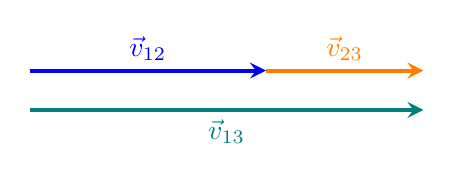
\begin{tikzpicture}
				\draw[-stealth, blue, line width=1.5pt] (0,0)--(3,0);
				\draw[-stealth, orange, line width=1.5pt] (3,0)--(5,0);
				\draw[-stealth, teal, line width=1.5pt] (0,-0.5)--(5,-0.5);
				\node[above, blue] at (1.5,0) {$\vec{v}_{12}$};
				\node[above, orange] at (4,0) {$\vec{v}_{23}$};
				\node[below, teal] at (2.5,-0.5) {$\vec{v}_{13}$};
			\end{tikzpicture}&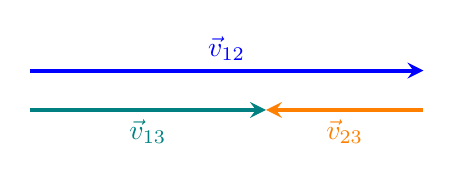
\begin{tikzpicture}
			\draw[-stealth, blue, line width=1.5pt] (0,0)--(5,0);
			\draw[-stealth, orange, line width=1.5pt] (5,-0.5)--(3,-0.5);
			\draw[-stealth, teal, line width=1.5pt] (0,-0.5)--(3,-0.5);
			\node[above, blue] at (2.5,0) {$\vec{v}_{12}$};
			\node[below, orange] at (4,-0.5) {$\vec{v}_{23}$};
			\node[below, teal] at (1.5,-0.5) {$\vec{v}_{13}$};
			\end{tikzpicture}&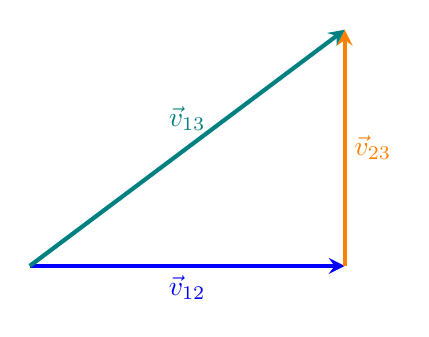
\begin{tikzpicture}
			\draw[-stealth, blue, line width=1.5pt] (0,0)--(4,0);
			\draw[-stealth, orange, line width=1.5pt] (4,0)--(4,3);
			\draw[-stealth, teal, line width=1.5pt] (0,0)--(4,3);
			\node[below, blue] at (2,0) {$\vec{v}_{12}$};
			\node[right, orange] at (4,1.5) {$\vec{v}_{23}$};
			\node[above, teal] at (2,1.6) {$\vec{v}_{13}$};
			\end{tikzpicture}\\
			 $v_{13}=v_{12}+v_{23}$&$v_{13}=\left|v_{12}-v_{23}\right|$&$v^2_{13}=v^2_{12}+v^2_{23}$
		\end{tabular}
		
	\end{center}
	HS trình bày kết quả ví dụ 1:\\
	Câu trả lời dự kiến:
	\begin{enumerate}[label=\alph*)]
		\item Hành khách đi từ cuối tàu đến đầu tàu: $v_{13}=v_{12}+v_{23}=\SI{71}{\meter/\second}$.
		\item Hành khác đi từ đầu tàu đến cuối tàu $v_{13}=\left|v_{12}-v_{23}\right|=\SI{69}{\meter/\second}$.
	\end{enumerate}
}
{\textit{\underline{* GV chuyển giao nhiệm vụ học tập}}\\
	GV ôn tập lại quy tắc hình bình hành để cộng hai vector.\\
	GV giới thiệu mở rộng cho HS quy tắc tam giác vector.\\
	GV chia lớp thành 6 nhóm.\\
	GV yêu cầu HS hoạt động theo nhóm, áp dụng quy tắc tam giác vector để xác định độ lớn vận tốc tổng hợp trong 3 trường hợp đơn giản.\\
	GV chuyển giao HS thực hiện ví dụ 1.\\
	\textit{\underline{* HS thực hiện nhiệm vụ học tập}}\\
	HS tích cực trao đổi theo nhóm.\\
	GV quan sát, hỗ trợ các nhóm gặp khó khăn.\\
	\textit{\underline{* HS báo cáo kết quả thực hiện nhiệm vụ học tập}}\\
	GV mời đại diện 3 nhóm lên bảng trình bày cho 3 trường hợp.\\
	Các nhóm còn lại nhận xét, góp ý.
	\\
	GV mời 2 HS lên bảng trình bày kết quả ví dụ 1.
	\\
	GV chỉnh lí, hợp thức hóa kiến thức.
}
\hoatdong{
	Luyện tập.
}
{
	HS xác định được vận tốc tổng hợp.\\
	HS giải được bài tập thuyền chuyển động xuôi dòng/ngược dòng.
}
{
	Bài tập cá nhân của học sinh.
}
{
	\textit{\underline{GV chuyển giao nhiệm vụ học tập}}\\
	GV lần lượt chuyển giao từng bài tập, yêu cầu HS hoạt động cá nhân để giải.\\
	\textit{\underline{HS thực hiện nhiệm vụ học tập}}\\
	HS \textit{(làm việc cá nhân)}:  Giải bài tập trong phiếu bài tập được GV giao. 
	
	GV: Theo dõi để phát hiện các HS gặp khó khăn, từ đó đưa ra sự định hướng, hỗ trợ phù hợp cho mỗi HS.\\
	\textit{\underline{HS báo cáo kết quả thực hiện nhiệm vụ học tập}}\\
	GV: Mời HS lên bảng giải bài tập.
	
	HS: Đặt câu hỏi, góp ý.
	
	GV: Chỉnh lí, hợp thức hoá kiến thức.
}
\section{HỒ SƠ DẠY HỌC}
\subsection{NỘI DUNG DẠY HỌC}
\begin{enumerate}[label=\bfseries\Roman*.]
	\item \textbf{TÍNH TƯƠNG ĐỐI CỦA CHUYỂN ĐỘNG}\\
	\begin{enumerate}[label=\bfseries\arabic*.]
		\item \textbf{Tính tương đối của vị trí}\\
		Trong các hệ quy chiếu khác nhau, vị trí của vật cũng khác nhau nên dạng quỹ đạo cũng khác nhau.
		\item \textbf{Tính tương đối của vận tốc}\\
		Trong các hệ quy chiếu khác nhau, vận tốc của vật khác nhau.
	\end{enumerate}
	$\Rightarrow$ \textbf{Vị trí và vận tốc của vật có tính tương đối.
	 }
	 \begin{itemize}
	 	\item \textbf{Hệ quy chiếu đứng yên} là hệ quy chiếu gắn với vật làm gốc được quy ước là đứng yên.
	 	\item \textbf{Hệ quy chiếu chuyển động} là hệ quy chiếu gắn với vật làm gốc chuyển động so với hệ quy chiếu đứng yên.
	 \end{itemize}
	 \item \textbf{ĐỘ DỊCH CHUYỂN TỔNG HỢP - VẬN TỐC TỔNG HỢP}\\
	 Xét vật 1 chuyển động so với vật 3 đứng yên (được chọn làm gốc của HQC đứng yên); vật 2 (được chọn làm gốc của HQC chuyển động) chuyển động so với vật 3. Ta có:\\
	 Khi vật 1 có độ dịch chuyển $\vec{d}_{12}$ so với vật 2, đồng thời vật 2 cũng có độ dịch chuyển $\vec{d}_{23}$ so với vật 3 và khi đó vật 1 có độ dịch chuyển $\vec{d}_{13}$ so với vật 3.\\
	 \textbf{Biểu thức độ dịch chuyển tổng hợp:}\\
	 $$\vec{d}_{13}=\vec{d}_{12}+\vec{d}_{23}$$
	 \textbf{Biểu thức của vận tốc tổng hợp:}
	 $$\vec{v}_{13}=\vec{v}_{12}+\vec{v}_{23}$$
	 \begin{center}
	 	\begin{tikzpicture}
	 		\coordinate (O) at (0,0);
	 		\coordinate (A) at ($(O)+(60:3)$);
	 		\coordinate (B) at (4,0);
	 		\coordinate (C) at ($(B)+(60:3)$);
	 		\draw[-stealth, line width=1.5pt, blue] (O)--(B);
	 		\draw[-stealth, line width=1.5pt, orange] (O)--(A);
	 		\draw[-stealth, line width=1.5pt, teal] (O)--(C);
	 		\draw[ line width=1.5pt, black, dashed] (A)--(C)--(B);
	 		\node[right, teal] at (C) {$\vec{v}_{13}$};
	 		\node[below, blue] at (B) {$\vec{v}_{23}$};
	 		\node[above left, orange] at (A) {$\vec{v}_{12}$};
	 	\end{tikzpicture}
	 \end{center}
	 Trong đó:
	 \begin{itemize}
	 	\item $\vec{v}_{13}$: vận tốc của vật 1 đối với vật 3, gọi là \textbf{vận tốc tuyệt đối};
	 	\item $\vec{v}_{12}$: vận tốc của vật 1 đối với vật 2, gọi là \textbf{vận tốc tương đối};
	 	\item $\vec{v}_{23}$: vận tốc của vật 2 đối với vật 3, gọi là \textbf{vận tốc kéo theo}.
	 \end{itemize}
	 \textbf{Các trường hợp đặc biệt:}
	 \begin{itemize}
	 	\item Trường hợp $\vec{v}_{12}$ và $\vec{v}_{23}$ cùng hướng: $v_{13}=v_{12}+v_{23}$;
	 	\item Trường hợp $\vec{v}_{12}$ và $\vec{v}_{23}$ ngược hướng: $v_{13}=\left|v_{12}-v_{23}\right|$;
	 	\item Trường hợp $\vec{v}_{12}$ và $\vec{v}_{23}$ vuông góc: $v^2_{13}=v^2_{12}+v^2_{23}$.
	 \end{itemize}
\end{enumerate}
\subsection{CÁC HỒ SƠ KHÁC}
\textbf{* Các câu hỏi ví dụ}\\
\setcounter{ex}{0}
% ======================================================================
\begin{ex}
	Bên trong một tàu lửa đang chuyển động thẳng đều với tốc độ $\SI{70}{\meter/\second}$, một hành khách di chuyển trong tàu với tốc độ $\SI{1}{\meter/\second}$ so với lái tàu. Xác định tốc độ của người đối với cột đèn tín hiệu bên đường trong trường hợp:
	\begin{enumerate}[label=\alph*)]
		\item hành khách đi từ cuối tàu đến đầu tàu.
		\item hành khách đi từ đầu tàu đến cuối tàu.
	\end{enumerate}
	
	\loigiai{\begin{enumerate}[label=\alph*)]
			\item Hành khách đi từ cuối tàu đến đầu tàu: $v_{13}=v_{12}+v_{23}=\SI{71}{\meter/\second}$.
			\item Hành khác đi từ đầu tàu đến cuối tàu $v_{13}=\left|v_{12}-v_{23}\right|=\SI{69}{\meter/\second}$.
	\end{enumerate}}
\end{ex}
% ======================================================================
\begin{ex}
	Hai bến A và B nằm dọc theo một con sông, cách nhau $\SI{6}{\kilo\meter}$. Khi nước đứng yên (không chảy) thì thuyền chạy với tốc độ $\SI{5}{\kilo\meter/\hour}$. Khi nước chảy  với tốc độ $\SI{1}{\kilo\meter/\hour}$ và động cơ của thuyền vẫn hoạt động như trước thì thời gian thuyền chuyển động từ A đến B rồi trở lại A là bao nhiêu? Giả sử bỏ qua thời gian thuyền quay đầu.
	
	\loigiai{
	$\SI{2.5}{\hour}$.
	}
\end{ex}